\documentclass[../../../OAE-SPEC-MAIN.tex]{subfiles}
\begin{document}


 
\section{It takes Two to Tango, and Three to Party}

%\subsection{Alice, Bob, and Carol with 3 LINKs}

Because a single link between Alice and Bob can be causally disconnected by real-world, permanent or intermittent failures, an alternative: statistically--independent--failure--path is necessary, to recover from \LINK Failures.  % ADD MODAL LOGIC necessary, etc.
This is the heart of the  Æ \texttt{ATOMICITY} claim:   A local (one hop \LINK) \texttt{TRIANGLE}  is the minimum necessary.  See TRIANGLE Clocks later in this specification.

 \begin{marginfigure}
        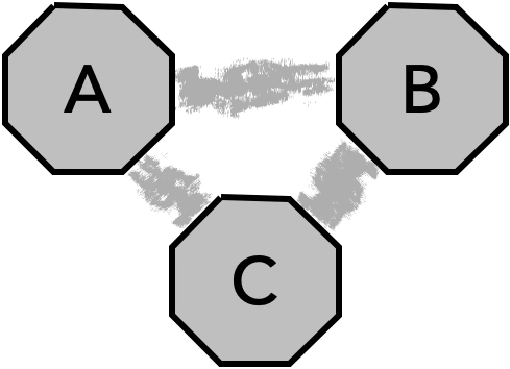
\includegraphics[width=\linewidth]{Tripartite-discovery.pdf}
  \caption{It takes three to party.  Links need an alternate path. This won't work over a Switched (Clos) Network.  
}
 %   \caption{A-B-C Flakey.pdf}
    \vspace{16pt}
\end{marginfigure}


%\subsection{\LINKs are Flakey}

 \begin{marginfigure}
      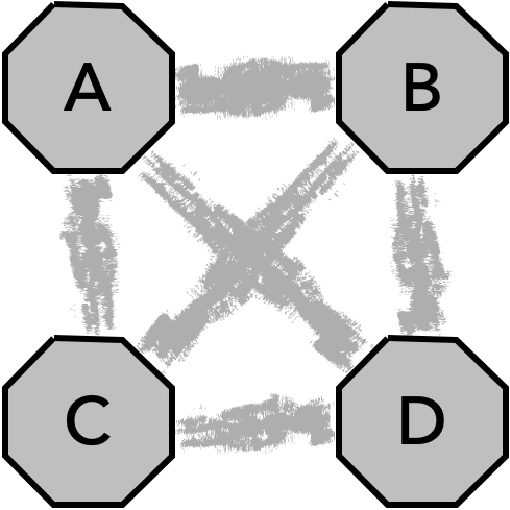
\includegraphics[width=\linewidth]{Quadpartite-discovery.pdf}
  \caption{2 x 2 =4  connected nodes with 6 flakey LINKs. Any one of which may be working in both directions: $\{11\}$, only one direction: $\{01\}$ or $\{10\}$, or \emph{not}-working in  \emph{both} directions: $\{11\}$. For 4 nodes, there are $\frac{(n(n-1)}{2} = 6$. With 4  \emph{reliability configurations} on each \LINK $\{00,01,10,11\}$ This gives us ONE correct (all links working correctly) and  $4^6-1 = 4095$ possible failure modes.}%\marginnote{permutations or combinations?} 
   \vspace{10pt}
\end{marginfigure}

\end{document}
